\chapter{Design}
\label{ch_design}

This chapter is dedicated to the various modules which comprise the laser tag system being investigated. The system is complex and comprises of many modules both in hardware and software. An overview of the entire system is given followed by the design of the individual modules.

It is important to reiterate at this point that this study aims determine the core components of a laser tag module with respect to the tagger and target system. The goal is not to design a ready to play 'user friendly' kit, but rather to determine what modules are required in such a system and how these components perform through the execution of various experiments.

\section{System Overview}

The hardware and software modules of the system will be addressed separately. Figure \ref{fig:system_overview_hardware} gives an overview of the hardware modules required to create a functional laser tag system.

\subsection{Hardware}

\begin{figure}[H]
	\centering
	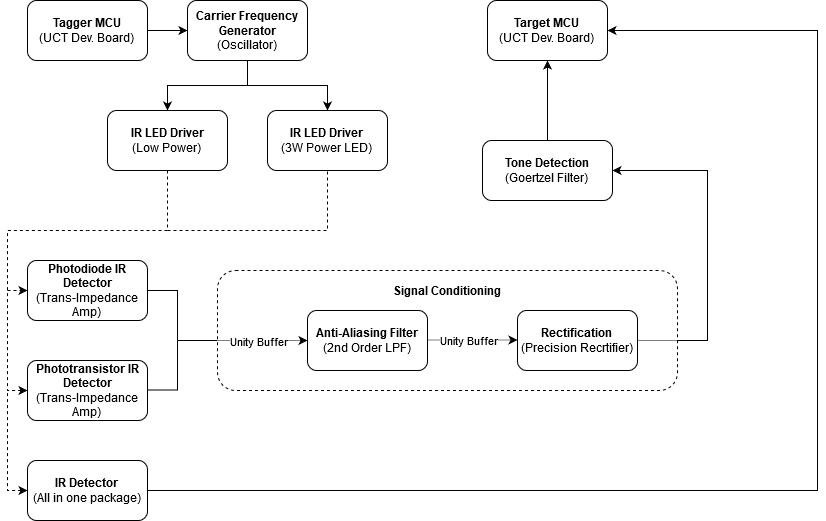
\includegraphics[width=0.9\textwidth]{figures/design/system_overview_hardware}
	\caption{Block Diagram of Hardware Modules}
	\label{fig:system_overview_hardware}
\end{figure}

\subsubsection{Tagger}
The tagger system, in terms of hardware, comprises of a main processor which has been realised on the UCT STM32\footnotemark{} development board. The main processor communicates with the carrier frequency generation module which is responsible for producing the 36kHz square waveform which feeds into the final hardware module of the tagger, the LED driver. Two led driver modules have been design, they both accept the same input signal and are identical in their purpose. The difference between the two modules is in the rated output power, the low power module is designed to drive a typical IR led while the high power module has been designed to drive a high power 3W IR led.

\footnotetext{STM32F051C6}

\subsubsection{Target}
The target system comprises many more hardware modules, this is due to the comparably higher complexity involved in detecting and processing signals. An additional module is also required to allow for a comparison between using a photodiode versus a phototransistor, as these each require a custom dedicated hardware module. The target system hardware consists of three IR sensors, in addition to the two sensors just mention, an 'all in one' IR receiver device was used to act as a golden measure against which to test the other two receivers. The output of the IR receiver module can be routed directly to the target main processor.

The outputs of the photodiode and phototransistor IR detection modules are routed into a signal conditioning module. This module performs anti-alias filtering and rectification of the signal, this is to ensure the signal is within the specifications of the tone detector. The tone detection modules comprises of a digital signal processing (DSP) algorithm, implemented on an STM32 MPU. The output of the tone detection module may be routed to the target main processor. The target main processor is implemented on the UCT STM32 development board.

\subsection{Software}

\begin{figure}[H]
	\centering
	%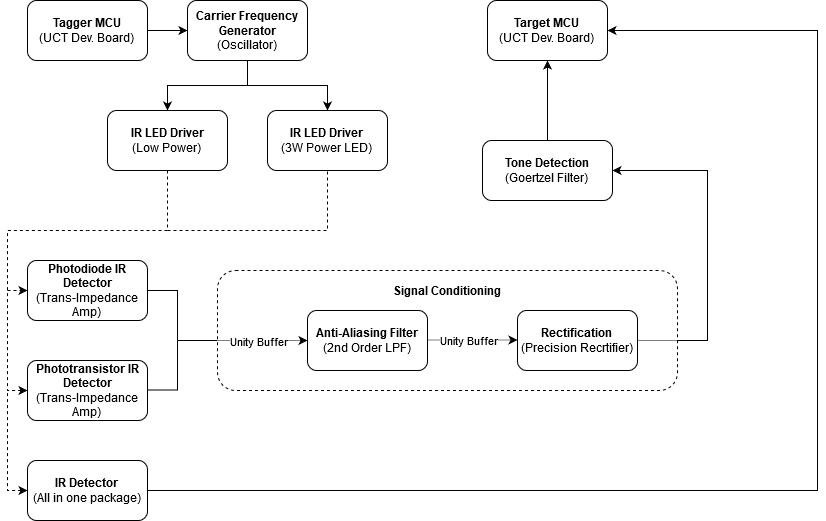
\includegraphics[width=0.9\textwidth]{figures/design/system_overview_hardware}
	\caption{Block Diagram of Software Modules}
	\label{fig:system_overview_software}
\end{figure}



\section{Hardware Modules}

\subsection{Tagger \& Target MCUs}
%Missing
% - Schematic and the like in the appendix
The laser tag systems has two main processors. One for the tagger and another for the target. The hardware used for main processor in each case is the UCT development board built around the STM32F051C6 microcontroller.

\begin{figure}[H]
	\centering
	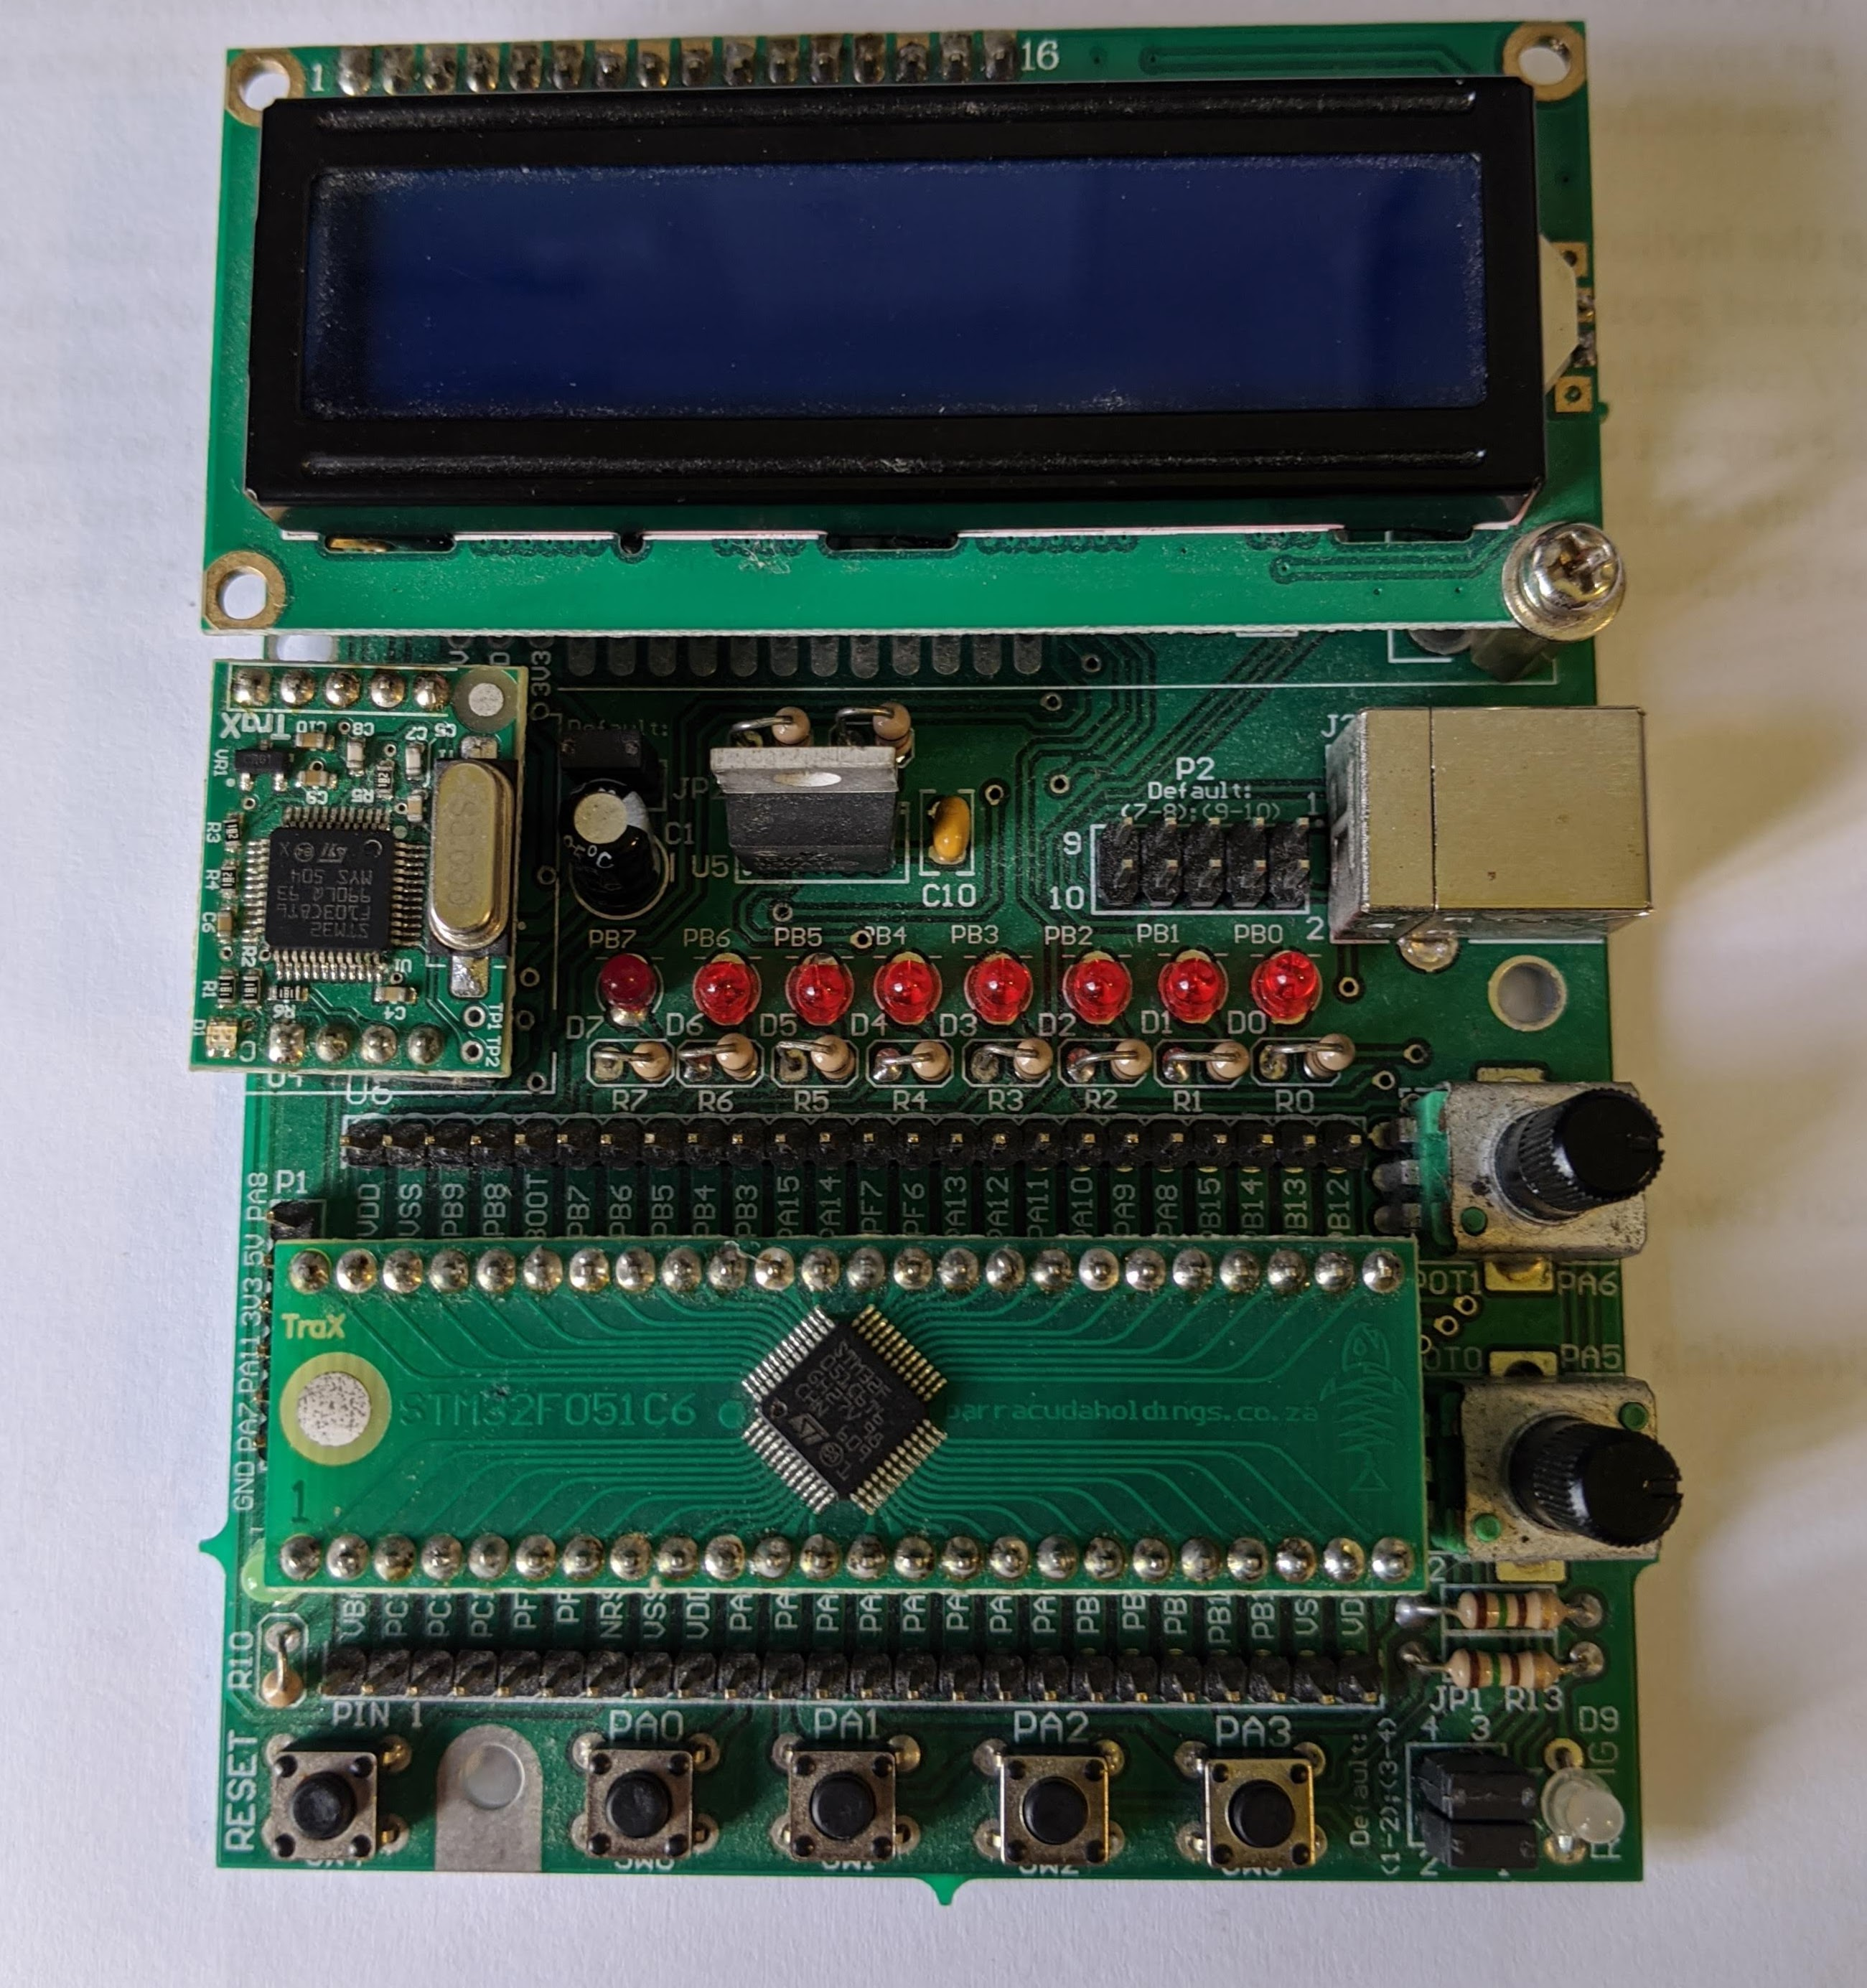
\includegraphics[width=.5\textwidth]{figures/design/dev_board_image.jpg}
	\caption{UCT STM32 Development Board}
	\label{fig:stm32_dev_board}
\end{figure}

The development board provides break-out pins for the microcontroller, 4 input buttons, an array of 8 LEDs, an LCD display and a built-in st-link v2 for debugging and programming the processor. 


\subsection{Carrier Frequency Generator}
%Missing
% - Calculations and chosen values
To generate the 36kHz carrier waveform the LM555 timer IC was used. The module is designed to receive a 3.3V logic control signal. The LED driver modules were designed to operate using an open-drain control signal, therefore a transistor was used to convert the push-pull output to an open-drain output. Figure \ref{fig:schematic_carrier_generation} shows the schematic for the module.


\begin{figure}[H]
	\centering
	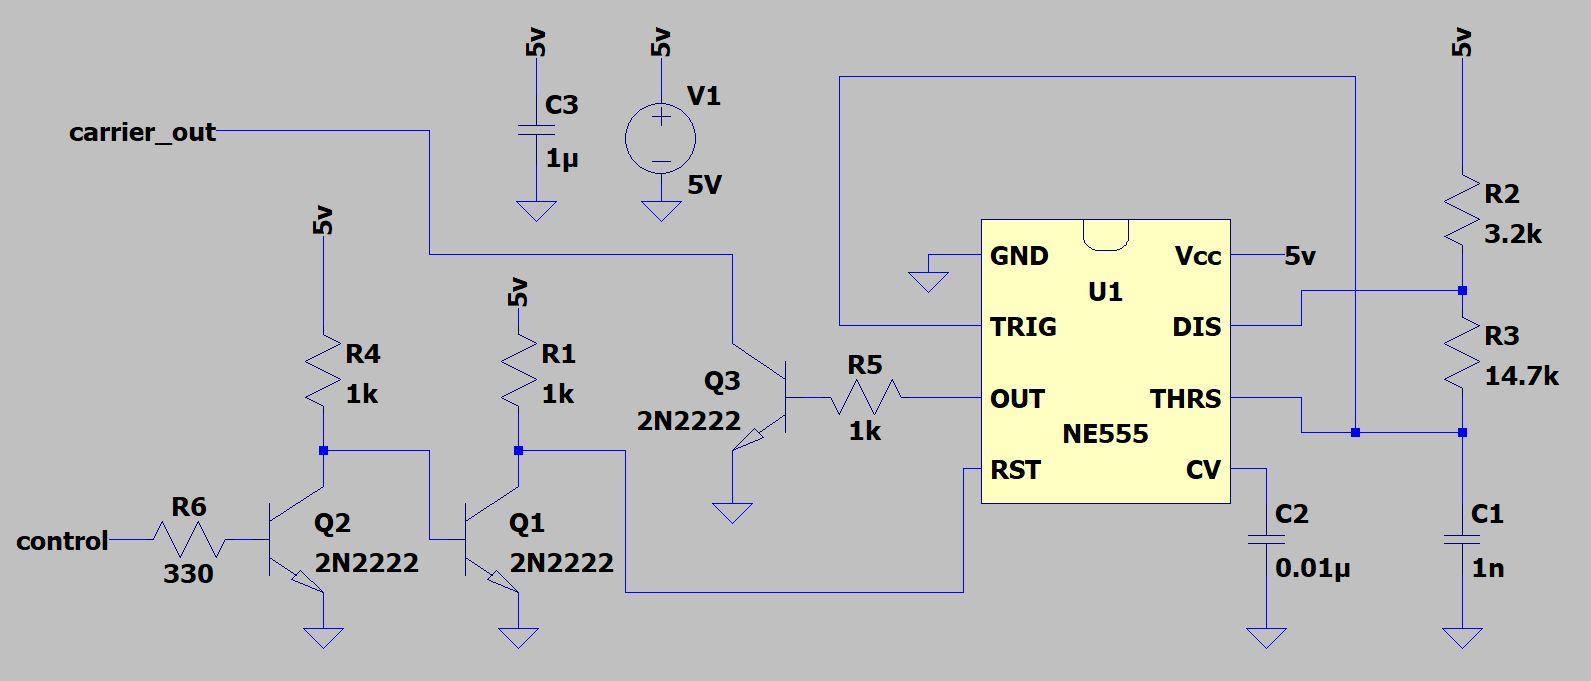
\includegraphics[width=.8\textwidth]{figures/design/carrier_waveform_generator_555.JPG}
	\caption{Carrier Generation Module Schematic}
	\label{fig:schematic_carrier_generation}
\end{figure}


\subsection{Power LED Driver}
%Missing:
% - Specs and component choice etc.

To operate the 3W high power IR LED a constant current driver module needed to be implemented. Because the LED needs to be modulated at 36kHz, standard LED drivers that use a switching regulator are not viable because the switching frequency requirements exceed those available in standard ICs.

\begin{figure}[H]
	\centering
	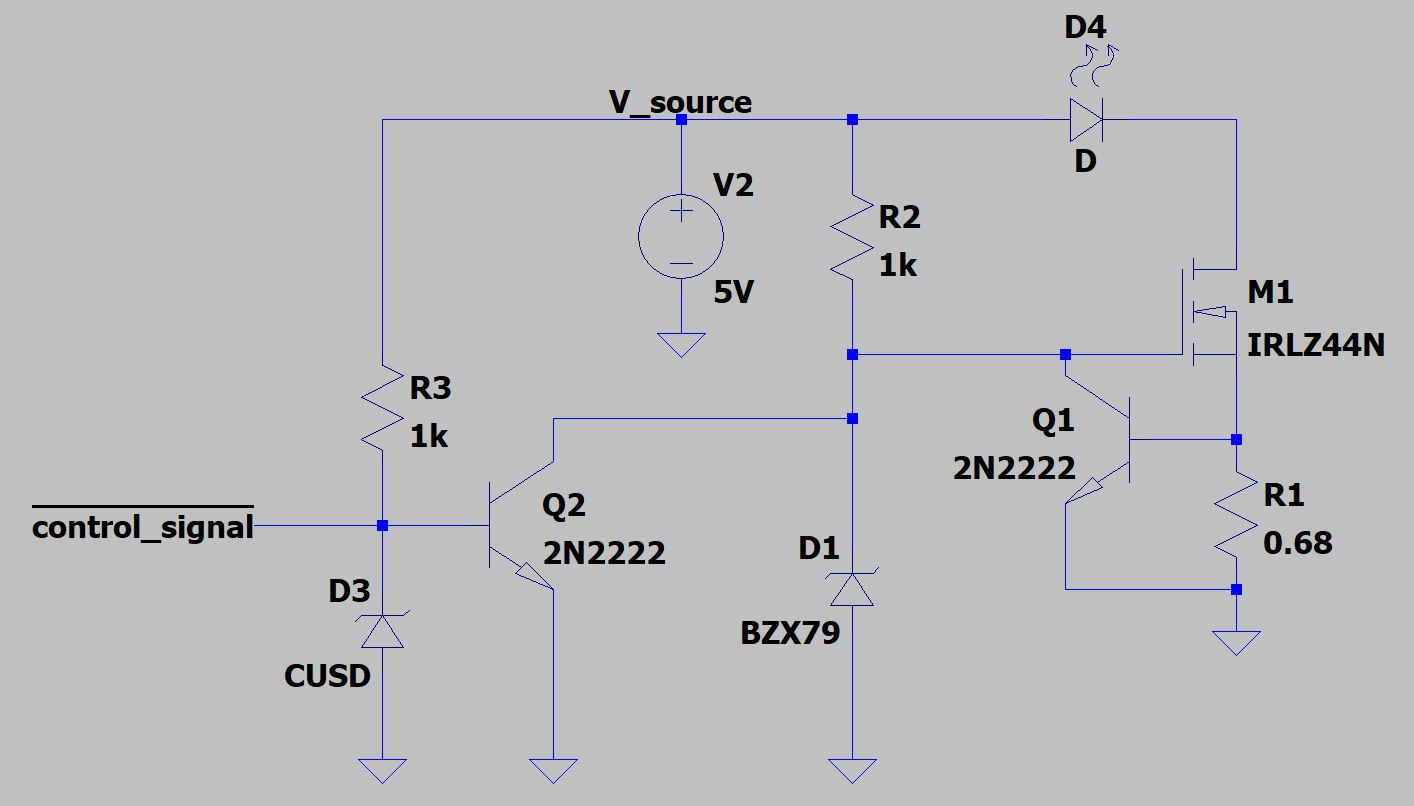
\includegraphics[width=.8\textwidth]{figures/design/power_led_driver.JPG}
	\caption{Power LED Driver Module Schematic}
	\label{fig:schematic_power_led_driver}
\end{figure}

Instead a linear regulator was designed. Figure \ref{fig:schematic_power_led_driver} shows the design of a high power linear regulator, built around the IRLZ44 enhancement PMOSFET. Heat-sinks where attached to both the high power LED and the IRLZ44 power MOSFET. However because the LED is only on for short bursts spread over sufficiently long time intervals it is likely that the heat-sinks are unnecessary.

The module is designed to be driven by an open-drain configured GPIO pin. By pulling the control signal low, the LED is powered and when the control signal is left floating the LED is powered off.

\subsection{Power LED Focus System}
%Missing:
% - ...

The high power IR LED has a wide beam angle, as it is designed for large area illumination. This is the opposite effect that is desired for a laser tag system. To rectify this, a focus system in the form of a light focusing tube was designed. This prevents light from spilling out the side and it focuses the beam to minimize dispersion over long distances.

\begin{figure}[H]
	\centering
	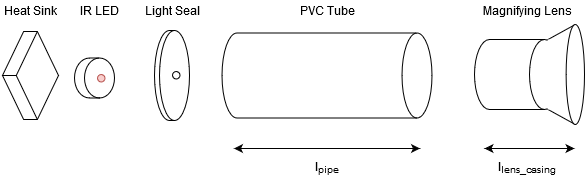
\includegraphics[width=.8\textwidth]{figures/design/beam_tube.png}
	\caption{Exploded View - Light Focusing Tube}
	\label{fig:light_focusing_tube}
\end{figure}

Figure \ref{fig:light_focusing_tube} above shows the components used to construct the light focusing tube. The length $l_{pipe}$ was determined by summing the experimentally calculated focal length of the lens with the length $l_{lens}$. Included in the calculation of the pipe length was the none-zero thickness of the light-seal (made out of 3mm hard-board) and the 3mm length of lens that remained external to the PVC piping.

The 40mm PVC piping used had a wall thickness of 2.3mm resulting in an inner diameter of 37.7mm. The magnifying lens had a length of 30mm and the lens is in-set by 1mm. The experimental result from section \ref{exp:focal_length} showed the focal length of the magnifying lens to be 53mm.

The length $l_{pipe}$ was calculated as follows

\[l_{pipe} = l_{lens} - l_{lens\_external} + l_{focal} - l_{light\_seal\_thickness} + l_{lens\_in-set\_distance}\]
\[l_{pipe} = 30mm - 3mm + 53mm - 3mm + 1mm = 78mm\]

\subsection{LED Driver}
%Missing:
% - Specs and component choice etc.

Due to the high power demands of the 3W IR LED, it is much more appropriate to perform test and develop the communication protocol using a low power IR led. A driver module was designed for this specific purpose.

\begin{figure}[H]
	\centering
	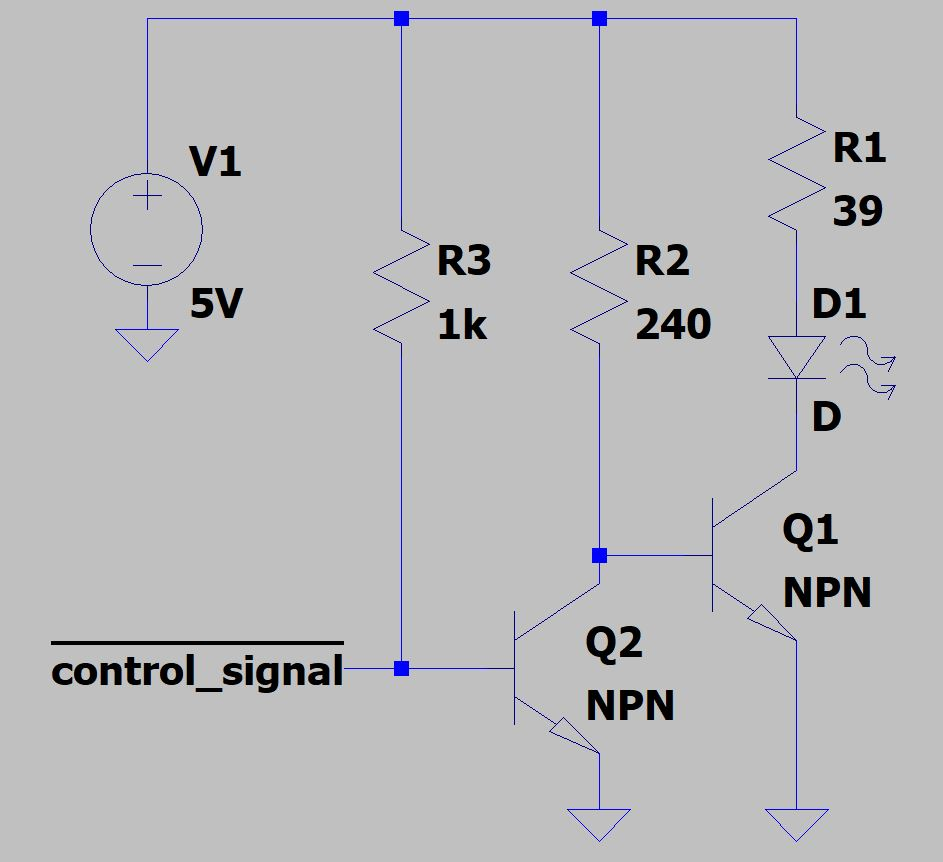
\includegraphics[width=.6\textwidth]{figures/design/low_power_led_driver.JPG}
	\caption{Low-Power LED Driver Module Schematic}
	\label{fig:schematic_low_power_led_driver}
\end{figure}

Figure \ref{fig:schematic_low_power_led_driver} shows the schematic for this driver module. The module is designed to be driven using an open-drain configured GPIO pin so that it is 'drop-in' compatible with the high power driver module.

\subsection{Photodiode IR Detector}
%Missing:
% - Schematic and explaination
% - Talk about MCP6022 and important specs

The photodiode IR detector module is designed to detect changes in infrared radiation and convert these fluctuations into a voltage signal.

\begin{figure}[H]
	\centering
	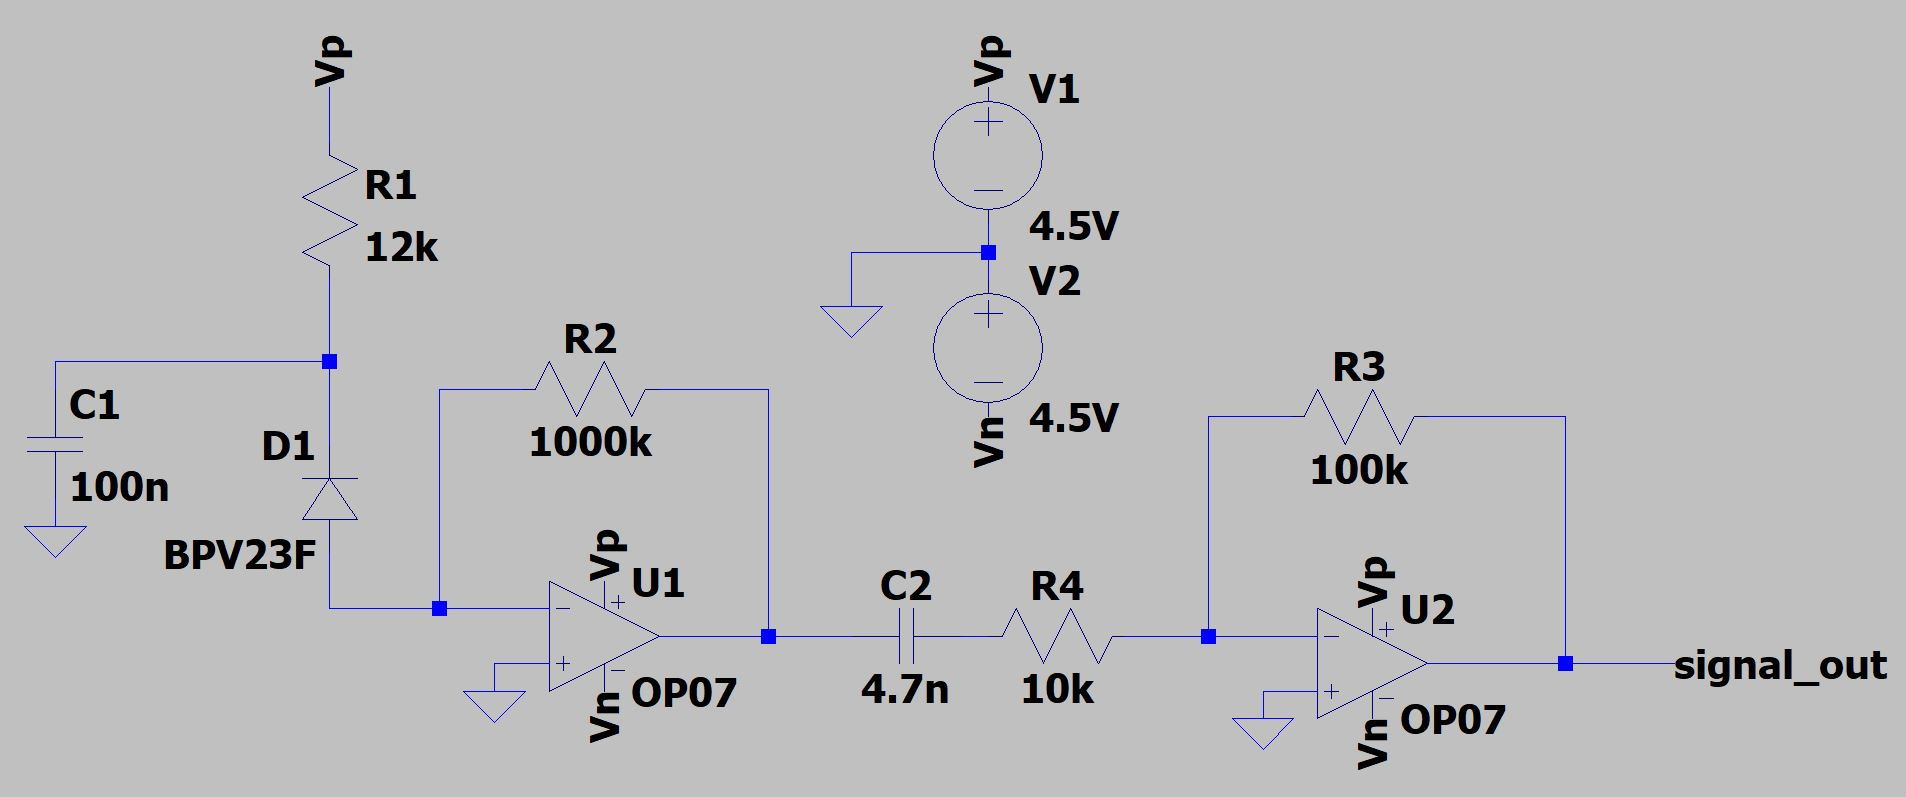
\includegraphics[width=.8\textwidth]{figures/design/photodiode_transimpedance.JPG}
	\caption{Photodiode IR Detector Module Schematic}
	\label{fig:schematic_photodiode_transimpedance}
\end{figure}

The circuit shown in figure \ref{fig:schematic_photodiode_transimpedance} is designed to produce a voltage in proportion to the current flowing through the photodiode. The circuit is inspired by S. Schrires 'Infrared Radio Link' circuit which is found in the EEE3071 course notes\cite{Schrire2007}.

\subsection{Phototransistor IR Detector}
%Missing:
% - Schematic and explaination


The phototransistor IR detector module is designed to detect changes in infrared radiation and convert these fluctuations into a voltage signal.

\subsection{IR Detector}
%Missing:
% - Schematic and explaination

The IR receiver is an 'all in one package' detector IC designed to detect the presences of a carrier signal in the IR light incident on the detector.

\begin{figure}[H]
	\centering
	\begin{minipage}{.5\textwidth}
		\centering
		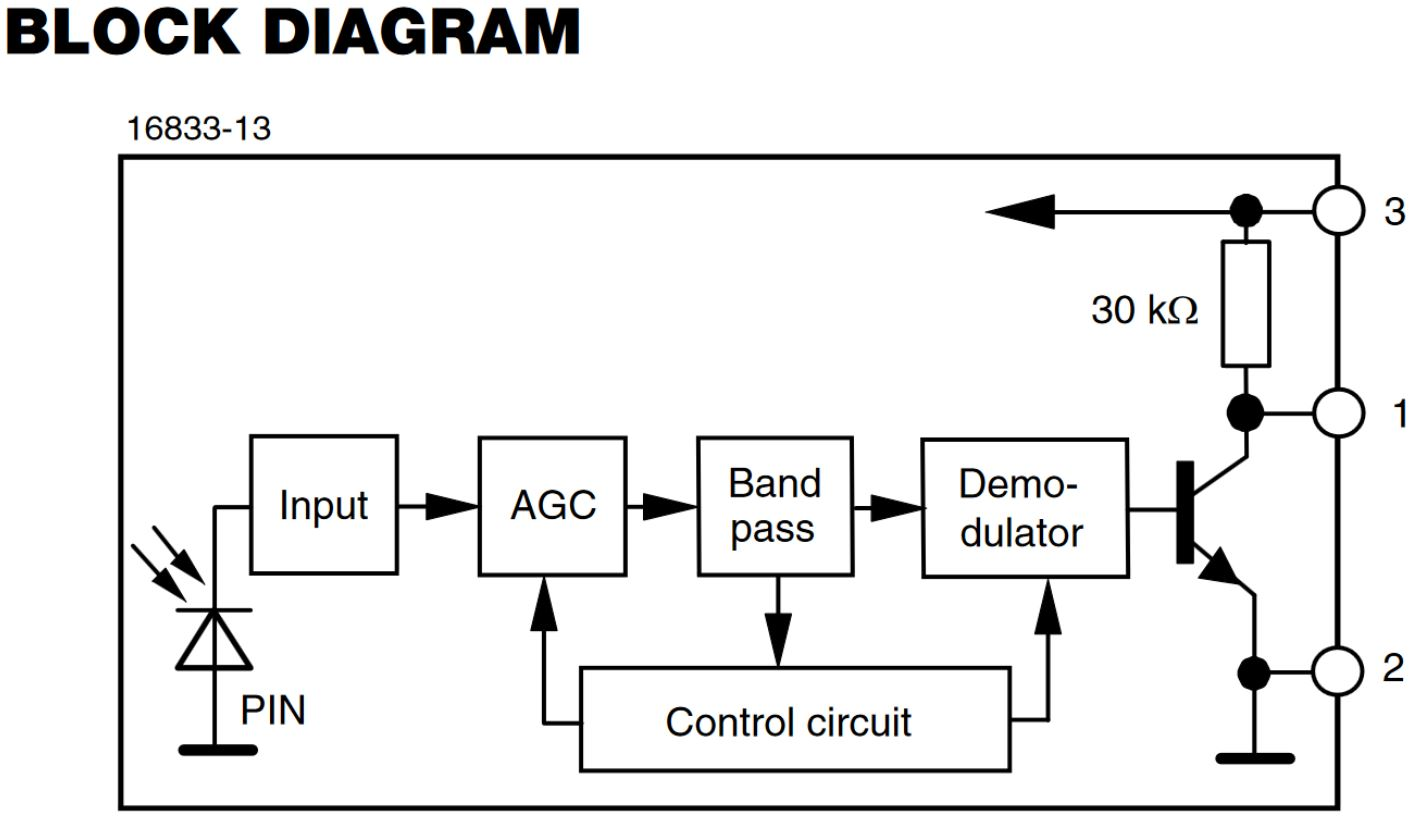
\includegraphics[width=.8\linewidth]{figures/design/TSOP382_block_diagram}
		\captionof{figure}{TSOP382 Functional Diagram}
		\label{fig:tsop382_block_diagram}
	\end{minipage}%
	\begin{minipage}{.5\textwidth}
		\centering
		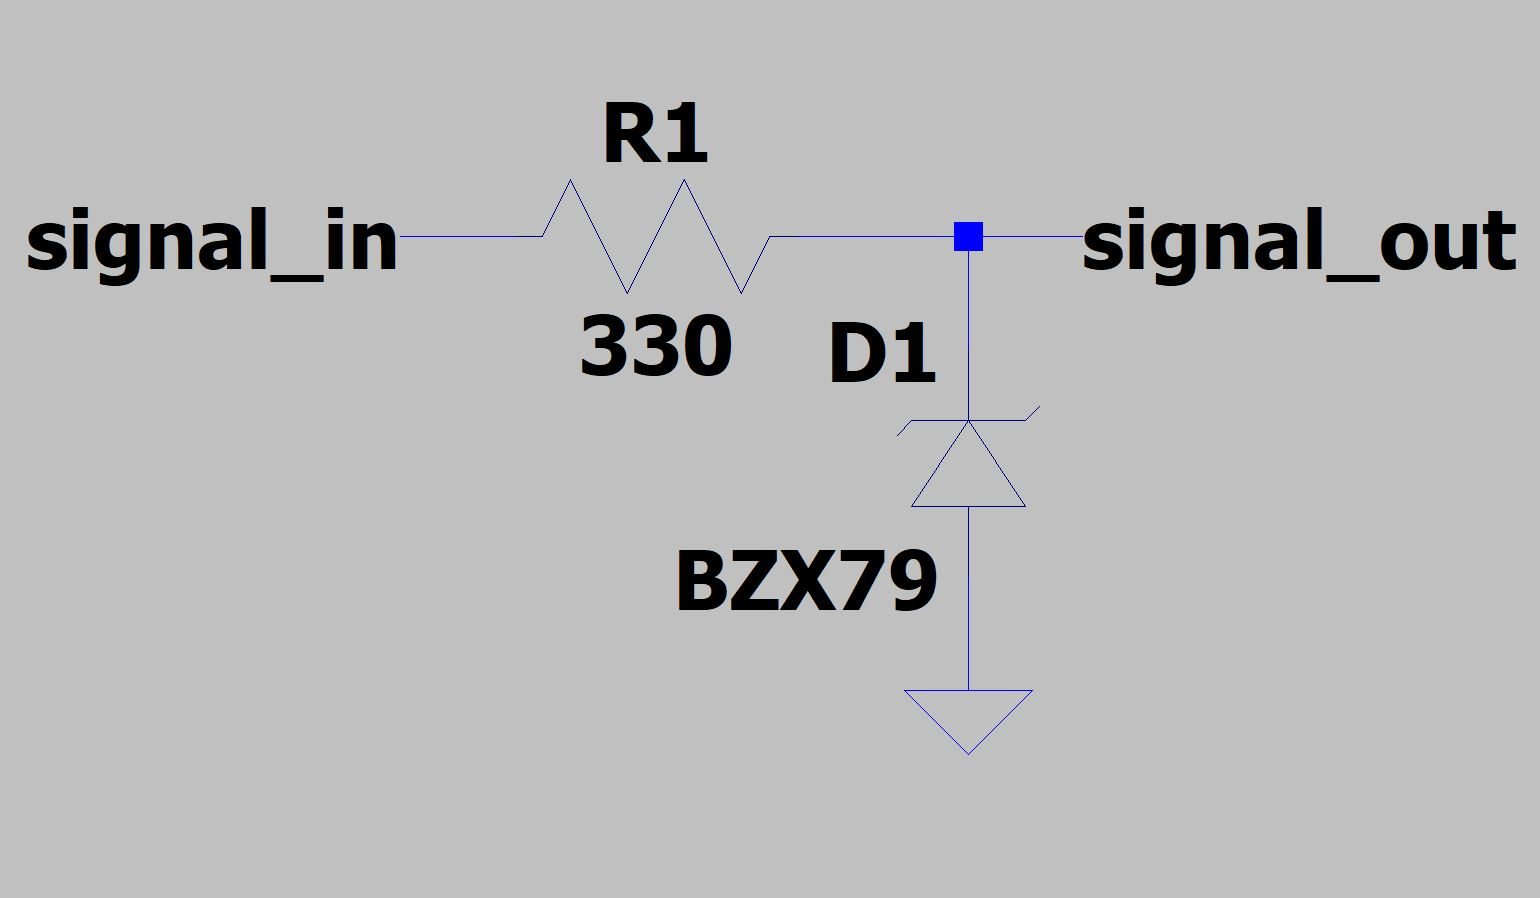
\includegraphics[width=.8\linewidth]{figures/design/over_voltage_protection}
		\captionof{figure}{Voltage Clamp}
		\label{fig:schematic_voltage_clamp}
	\end{minipage}
\end{figure}

The IR receiver used in this investigation is the TSOP382 from Vishay. The \href{https://www.vishay.com/docs/82491/tsop382.pdf}{datasheet} contains a block diagram (shown in figure \ref{fig:tsop382_block_diagram}) which gives a functional overview of the IC.

Figure \ref{fig:schematic_voltage_clamp} shows the circuity used to clamp the output of the IR receiver at 3V. This is to protect the GPIO from an over-voltage. The TSOP382 may be powered off 3.3V which would remove the voltage clamp requirement, however it has been included to ensure the module can be powered with a range of supply voltages and still be logically compatible with the STM32.

\subsection{Signal Conditioning Module}
%Missing:
% - Choosing freq cut off and what is expected gain

Before the voltage signal from the photodiode IR detector can be processed by the tone detector, it must be conditioned. The module can be broken into two stages separated by the unity buffer (U4). The first stage of the module performs filtering, this is prevent aliasing during the digital signal processing, which occurs when frequencies greater than half the sampling frequency are present in the sampled waveform. The second stage performs precision rectification, the signal is rectified to ensure a negative voltage is not placed on the input pin of the tone detector which is only tolerant of positive voltages between 0V and 3.3V.

\begin{figure}[H]
	\centering
	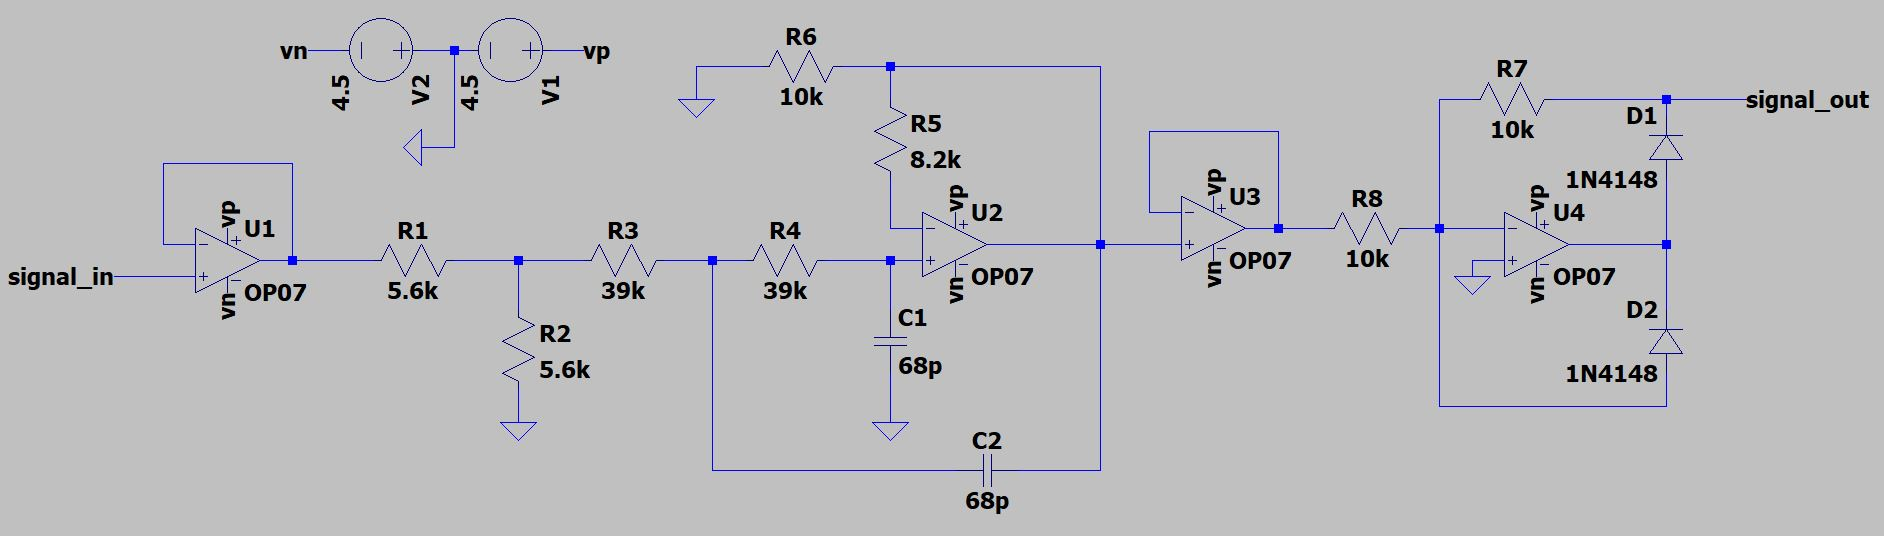
\includegraphics[width=\textwidth]{figures/design/filter_and_rectify}
	\caption{Signal Conditioning Module Schematic}
	\label{fig:schematic_filter_and_rectify}
\end{figure}

Often the incoming signal is a square wave with an amplitude of 4.5V which saturates the op-amps, to prevent saturation a voltage divider is formed using R1 and R2 to reduce the signal magnitude under these circumstances.

The filter circuit used is a second order voltage controlled voltage source (VCVS) active low pass filter in a Chebyshev configuration. The component values where chosen in acordances to the filter design table found on page 274 of the book 'The art of electronics'\cite{Horowitz1995}.

The precision rectifier is also a circuit design taken from the book and can be found on page 188, it is an improved version of the basic precision rectifier because it reduces the output swing of the op-amp during operation\cite{Horowitz1995}.

\subsection{Tone Decoder Module}
%Missing:
% - Is a schematic worth the bother?

The tone decoder module's hardware consists of an STM32F051C6 breakout PCB which is mounted on a strip-board along with supporting circuity (external crystal and voltage regulation). In addition to the supporting circuitry, an over-voltage protection clamp (see figure \ref{fig:schematic_voltage_clamp}) was placed on pin 17 which is connected internally to PA7 which is configured as an analog input. Three signal LED's where wired to pins 18, 19 and 20 to act as status indicators.

The DSP algorithm is discussed in subsection \ref{tone_decoder_software} from the following section on software modules.






\section{Software Modules}

\subsection{Tone Decoder Module}
\label{tone_decoder_software}

In section \ref{sec:goertzel_implementation} the goertzel algorithm is given. The parameters k (the DFT frequency bin) and N (the number of samples per frequency bin coefficient calculation) determine the value of omega which in turn affects the value of 'cosval', 'sinval' and 'coeff'. The value of k is also affected by the ratio of the frequency of the k\textsuperscript{th} DFT frequency bin to the sampling frequency (f\textsubscript{sampling}).

The STM32F0 is designed to be low cost 32-bit microcontroller and utilizes the ARM Cortex-M0 CPU core. To reduce costs, this microcontroller does not contain any dedicated DSP peripherals nor does it contain any hardware dedicated to floating point arithmetic. Therefore careful consideration must be taken during design to optimize the performance of the goertzel filter implementation. The STM32F0 is equipped with several timers, a DMA peripheral and an advanced interrupt controller, these peripherals are indispensable for the implementation of the real-time digital filter. Figure \ref{fig:goertzel_functional_diagram} shows the functional blocks for the goertzel filter, the flow of data and clock signals.

\begin{figure}[H]
	\centering
	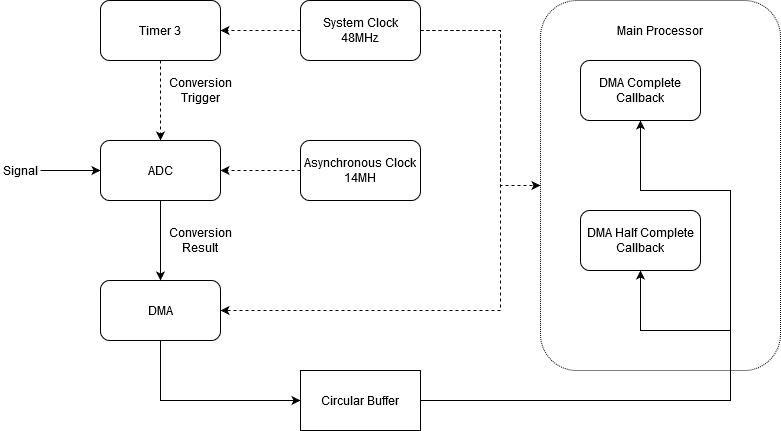
\includegraphics[width=.8\textwidth]{figures/design/goertzel_filter_functional.png}
	\caption{Goertzel Filter Functional Block Diagram}
	\label{fig:goertzel_functional_diagram}
\end{figure}

\subsubsection{Sampling Frequency Constraints}
\label{sec:sampling_frequency_constraints}
The sampling frequency determines the highest frequency that may be present in the sampled waveform before aliasing will occur. The higher the sampling rate, the wider the bandwidth of the goertzel filter. A higher sampling frequency also results in relaxed requirements for the antialiasing filter.

The sampling frequency is limited however by the speed of the microcontroller. This limitation influences the sampling frequency directly by acting as an upper bound to the rate at which the ADC can process and store each analog reading, however more critically, the sampling frequency is directly proportional to the number of samples that must be processed per period. Therefore it is necessary to keep the sampling frequency as low as possible.

\subsubsection{Filter Optimization}
\label{sec:filter_optimization_design}
As outlined at the beginning of this section, the most critical means of optimization for this filter is the full utilization of available peripherals. After reset, the main processor configures the timer, ADC and DMA to continuously sample the incoming signal and store the conversion results in a circular buffer. After this configuration, the main processor is freed from this process and all processing cycles are dedicated to processing the data being stored in the circular buffer.

The second means of optimization was realised after examination of the goertzel algorithm. By carefully engineering the configurable parameters in the goertzel algorithm (listing \ref{lst:goertzel_algorithm}) it is possible to reduce the computation time of the algorithm by removing the multiplication requirement for each new sample (line 13). This is achieved be choosing parameters that result in omega having a value of \(\frac{\pi}{2} + 2\pi m,\; m\epsilon \mathbb{Z}\) and as a consequence make 'cosval' and 'coeff' equal to zero.

It is important to note, this optimization does not improve the time complexity of the algorithm, in both cases the algorithm has a time complexity of O(N). However for real-time algorithms such as in the case of a goertzel filter, every possibly time saving is valuable and can be the difference between a working and failed implementation.

Line 4 of the algorithm provides the relationship between k, N and $\omega$

\begin{equation}
	\omega = \frac{2\pi * k}{N}
\end{equation}

Substituting \(\omega = \frac{\pi}{2} + 2\pi m,\; m\epsilon \mathbb{Z}\) and simplifying shows

\begin{equation}
\label{eqn:k_N_constraint}
	\frac{k}{N} = \frac{1+4m}{4},\; m\epsilon \mathbb{Z}
\end{equation}

If only integer values for k, N, $f_{sampling}$ and $f_{bin}$ are considered, line 3 of the algorithm provides the relationship between these parameters which may be expressed by the following equation

\begin{equation}
\label{eqn:k_N_and_fb_fs}
	\frac{k}{N} = \frac{f_{bin}}{f_{sampling}}
\end{equation}


Equation \ref{eqn:k_N_and_fb_fs} shows that the ratio of $f_{bin}$ to $f_{sampling}$ must be equal to that of k to N. This relationship reveals that the only realisable value for m is zero. Any value of m greater than zero requires a sampling frequency lower than the bin frequency which violates the Nyquist criteria and a negative value of m would require (for $f_{bin} \approx 36kHz$) a negative sampling frequency which is nonsensical. Therefore the final relationship between the ratios may be summarised in the following equation

\begin{equation}
\label{eqn:k_N_and_fb_fs_ratio}
\frac{k}{N} = \frac{f_{bin}}{f_{sampling}} = \frac{1}{4}
\end{equation}

Even after the above two means of optimizing the goertzel algorithm, the STM32F0 was not fast enough to process every sample. This is because even after optimizing the algorithm, it cannot processing incoming samples faster than the required 144kHz. The solution is to sample more than N samples per interrupt and drop the excess samples. This increases the amount of processing time per sample, but increases the latency between the filter's input and the output. This technique only works if the duration of modulation is much greater than the duration of samples dropped.

\subsubsection{Practical Implementation}

The desired bin frequency is 36kHz, according to equation \ref{eqn:k_N_and_fb_fs_ratio} this requires a sampling frequency of 144kHz. This is within the constraints set out in section \ref{sec:sampling_frequency_constraints}.

The ADC conversions are triggered by timer 3, a general purpose 16-bit timer. The timer accepts a pre-scalar and counter period value. The frequency of the timer's output and as a result the sampling frequency is given by \(f_{sampling} = \frac{f_{system\_clock}}{prescaler \times cperiod}\). Substituting our system clock frequency, desired sampling frequency and rearranging the equation we find the product of the pre-scalar and clock period values.

\[prescaler \times cperiod = \frac{48 \times 10^6}{144 \times 10^3} = 333.\dot{3}\]

The result, $333.\dot{3}$ cannot be formed as the product of two integer values, instead the closest integer value of 333 is used. Because this is well below the maximum value of the 16-bit counter period register, the pre-scalar is set to one. The resulting sampling frequency is $144.\dot{1}4\dot{4}$ kHz. Returning to equation \ref{eqn:k_N_and_fb_fs_ratio}, we see that we must choose $f_{bin} = 36.036$kHz to preserve the ratio required for optimization.


\subsection{Tagger Software}
%HERE






\subsection{Target Software}










